\section{Sistema de Refrigeração}

\section{Sistema de Alimentação}
As fontes de energia que serão utilizadas para alimentar o produto, incluindo o sistema de refrigeração e os componentes elétricos e eletrônicos, são a rede elétrica comum brasileira e um banco de baterias. O banco de baterias será dimensionada a fim de manter os subsistemas em perfeita operação durante o período solicitado de 48 horas.

\subsection{Diagrama do Sistema}
A Figura a seguir apresenta o diagrama elétrico simplificado do produto. Ele representa o circuito de alimentação utilizado, desde a fonte de energia --- rede elétrica padrão --- até o uso final em seus componentes elétricos e eletrônicos.  É importante ressaltar que este diagrama será refinado ao longo dos pontos de controle, pois o  sistema pode ser retificado para melhor atender às condições de contorno que forem encontradas durante a execução do projeto.

\begin{figure}[H]
\begin{center}
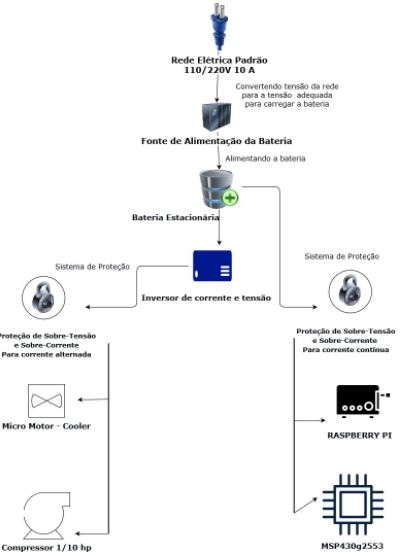
\includegraphics[scale = 1.2]{figuras/Diagrama_Simp.JPG}
\caption{ Diagrama Elétrico Preliminar}
\end{center}
\end{figure}

O sistema foi dimensionado com um fator de segurança elevado, pois a proposta de projeto é de um sistema de acondicionamento de órgãos para transplante. Sendo assim, o nível de confiabilidade do produto deve ser extremamente alto, para isso todo o sistema de alimentação foi dimensionado relacionando o sistema ao tempo de operação necessário ao transporte e diretamente ao consumo de energia advinda da bateria.


\subsection{Dimensionamento das Baterias}
	Baterias têm a finalidade de armazenar energia e liberá-la em determinada periodicidade, e de forma controlada. Sua escolha deve ser adequada às necessidades de consumo energético do projeto, e considera os dados de corrente elétrica e tensão. Para a seleção da bateria adequada deve-se estudar se ela é capaz de armazenar a energia total demandada às necessidades do projeto, e se ela consegue entregar toda a energia necessária ao funcionamento do equipamento. O processo de dimensionamento do banco de baterias deve ser realizado inicialmente e depois sucessivamente aperfeiçoado, em função dos demais dimensionamentos e ajustado em função dos custos, disponibilidade de mercado, entre outros.

	O processo de dimensionamento deve seguir algumas etapas, a primeira delas é definir o tipo de bateria a ser utilizado. Dentre as opções de bateria disponíveis no mercado, optou-se pela bateria estacionária. Sua vida útil é de aproximadamente 5 anos, devido à sua composição com materiais internos mais sobres se comparada às baterias automotivas, por exemplo. Podem, também, suportar descargas de até 80\% de sua capacidade, sem prejudicar sua vida útil, e resistem a ciclos de carga ou descarga mais profundos. Tais características proporcionam maior confiabilidade ao funcionamento do projeto pelo uso da bateria estacionaria.
	
	Após a escolha do tipo de bateria, deve ser analisada a profundidade de descarga com que se vai trabalhar. Quanto mais profundos os ciclos de descarga-carga, menor a vida útil da bateria. Ou seja, reduzir-se a capacidade da bateria, gasta-se menos no início, porém as baterias durarão menos e os gastos com reposição serão maiores. Um valor usado para essa profundidade de descarga para ciclos diários com baterias de chumbo-ácido é de 10\% a 20\%. Para ciclos esporádicos, podem ser utilizados ciclos mais profundos, da ordem de 60\%. 
	
	A capacidade do banco de baterias em Ah pode ser calculada conforme a expressão abaixo: 
	
	\begin{equation}
	Capacidade(Ah) = \frac{Consumo(\frac{Wh}{dia}) \times Autonomia(dias)}{V_{Baterias}(V)\times profundidade(pu)}
	\end{equation}

O dimensionamento da bateria requer inicialmente a relação de potência demandada para suprir as necessidades dos componentes elétricos do projeto, como mostra a tabela a seguir:

\begin{table}[H]
\caption{Consumo energético dos componentes}
\begin{tabular}{|p{4 cm} |c |c |c |}
 \hline
   \textbf{COMPONENTE} &\textbf{ALIMENTAÇÃO (V)}  &\textbf{CORRENTE (A)} & \textbf{POTÊNCIA (W)} \\
   \hline
  \textbf{MSP430g2553} &5 & 330$\mu$& 1,65 mW \\
   \hline
   \textbf{RASPBERRY PI}&5 &2,5 & 12,5 \\
   \hline
  \textbf{PROTETOR } &12 &26,5m &318m \\
   \hline
  \textbf{COMPRESSOR $\frac{1}{10}HP$} &12 & 2,4& 28,33 \\
   \hline
  \textbf{MICRO MOTOR} &12 &260,9m &3,6  \\
   \hline

\end{tabular}
\end{table}

Ao somar todas as cargas necessárias, o total foi de 229,819 Wh, já o consumo de corrente fica em 3,5365 A/h. O principal problema é o alto valor de partida do motor-compressor, o que é chamado de corrente de pico, no caso do motor-compressor utilizado, a corrente pode atingir um o valor entre 2-3 Ampères, o que requer atenção ao dimensionar a bateria para que ela suporte esse aumento inicial.


Com relação a profundidade da descarga no final da autonomia (pu) - utilizamos 0,6 (descargas mais profundas significam vida útil menor para a bateria e menos profundas um investimento inicial maior). Sendo que o consumo total é obtido a partir do levantamento das cargas, a autonomia de 5 horas.

Logo, 
$$
Capacidade \approx 33,2439 Ah
$$


\subsection{Dimensionamento do Inversor}
Inversores são conversores estáticos que, segundo Matakas Jr. E Komatsu (2011) transformam corrente ou tensão de forma contínua para a alternada. Muitos equipamentos operam em corrente/tensão contínua, sendo que a rede elétrica opera em corrente/tensão contínua. Portanto, a maneira mais simples de se trabalhar sem necessidade de mudanças drásticas em nenhum dos dois sistemas é se utilizar um inversor.

Este equipamento pode ser monofásico ou trifásico, sendo que o modelo utilizado no projeto será monofásico, e irá converter 12V da bateria que alimenta o sistema para 220V, valor de tensão que os outros componentes do sistema trabalham. Neste caso, com apenas duas chaves eletrônicas e uma fonte de tensão CC dividida é possível obter o inversor desejado.

Os inversores podem operar com duas tecnologias, senóide modificada ou senóide pura. No primeiro caso, formam uma onda quadrática, aproximando-se da senoidal AC, bom custo x benefício e pode ser aplicado na maioria dos casos, exceto para motores. O segundo caso pode ser usado como suprimento de energia AC em qualquer sistema, o que difere é o valor e o tamanho.

Um inversor bem dimensionado tem a potência maior que o consumo dos equipamentos para evitar que este trabalhe sempre em máxima potência,em suma um inversor é projetado em 3 estágios, oscilador, driver de corrente e transformador.
\begin{figure}[H]
	\begin{center}
		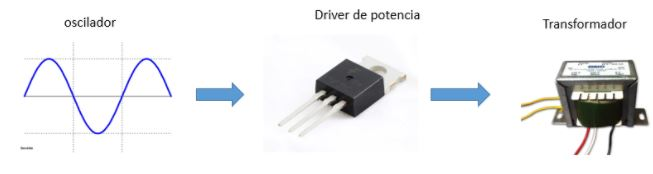
\includegraphics[scale = 0.75]{figuras/dim_inversor.JPG}
		\caption{ Diagrama Elétrico Preliminar}
	\end{center}
\end{figure}

Em primeiro lugar o oscilador transforma a corrente contínua em uma onda quadrada de 60Hz, que precisa ser adequada para uma onda senoidal, para isso é utilizado um filtro passa faixa centrado em 60Hz para eliminar as harmônicas indesejadas e obter uma onda senoidal mais eficaz possível. Entretanto, a saída do oscilador possui uma corrente muito baixa, por isso é necessário um ganho de corrente, para que seja entregue uma potência satisfatória na entrada do primário do transformador. Como a potência requerida é muito alta, se faz necessário que sejam inseridos vários transistores em paralelo para aumentar o ganho de corrente.

Na última fase o transformador faz a elevação da tensão para 220V que é a tensão necessária para ligar o compressor.

\subsection{Requisitos}
Com vistas à concepção e validação da solução, foram definidos os requisitos relativos ao subsistema de alimentação e refrigeração do produto:

\subsubsection{Requisitos Funcionais}
O sistema de alimentação deve ser capaz de:
\begin{itemize}
\item Armazenar energia elétrica;
 \item Fornecer energia para os componentes elétricos e eletrônicos de controle e monitoramento do produto;
 \item Fornecer energia para o sistema de refrigeração.
 \end{itemize}
\subsubsection{Requisitos Não Funcionais}
O sistema de alimentação deve ser capaz de:
\begin{itemize}
\item Prover a energia necessária para o bom funcionamento do produto durante um período máximo de 48 horas, com armazenamento de energia em baterias;
\item O sistema deve ser capaz de controlar a potência que será entregue as placas de peltier;
 \item Possuir eficiência energética aceitável, através de um controle de potência no sistema de refrigeração, escolha de componentes eletrônicos de baixa potência e sistemas de standby em determinados componentes não críticos do produto;
 \item Ser estável energeticamente, evitando picos de potência com componentes e segurança de circuitos.
 \end{itemize}